%!TEX root = ../tommaso-thesis.tex
%!TEX spellcheck = en_US


% status color definition
\definecolor{active}{HTML}{FF6600}
\definecolor{work needed}{HTML}{FF0000}
\definecolor{closed}{HTML}{888888}
\definecolor{resolved}{HTML}{666666}
\definecolor{working on}{HTML}{3388FF}
\definecolor{on hold}{HTML}{55FFFF}
\definecolor{unknown}{HTML}{D3D3D3}

\newcommand{\ie}{\textit{i.e.,}\xspace}
\newcommand{\eg}{\textit{e.g.,}\xspace}
\newcommand{\etc}{\textit{etc.}\xspace}
\newcommand{\etal}{\textit{et al.}\xspace}
\newcommand{\ib}{in*Bug\xspace}
\newcommand{\secref}[1]{Section~\ref{#1}\xspace}
\newcommand{\figref}[1]{Figure~\ref{#1}\xspace}
\newcommand{\tabref}[1]{Table~\ref{#1}\xspace}


\chapter{in*Bug: Visual Analytics of Bug Repositories}


Bug tracking systems are used to track and store the defects reported during the life of software projects. The underlying repositories represent a valuable source of information used for example for defect prediction and program comprehension. However, bug tracking systems present the actual bugs essentially in textual form, which is not only cumbersome to navigate, but also hinders the understanding of the intricate pieces of information that revolve around software bugs.\\
We present in*Bug, a web-based visual analytics platform to navigate and inspect bug repositories. in*Bug provides several interactive views to understand detailed information about the bugs and the people that report them. \\
% The tool can be downloaded at \textit{http://inbug.inf.usi.ch}

%%%%%%%%%%%%%%%%%%%%%%
\section{Introduction}
%%%%%%%%%%%%%%%%%%%%%%

Due to the complexity and size of non-trivial software projects, the development of a system is always accompanied by software defects, or bugs. To manage these defects, modern software projects use bug tracking systems (also known as bug trackers or issue trackers), such as Jira or Bugzilla. With bug trackers, end users and developers can report bugs they encountered while using the system, usually by means of custom web interfaces, where one can enter details about a specific bug, creating a so-called \emph{bug report}. A typical bug report, such as the one depicted in \figref{fogbugz-example}, contains information about \begin{inparaenum}[(1)] \item the title and id of the bug, \item the user who reported the bug and the people involved in its history, \item its current status, \item its opening and closing date, \item its last modification date, \item the project to which the bug report pertains, \item events (such as changes of the people assigned to the bug report, etc.) during the life cycle of the bug, etc. \end{inparaenum} The example bug report depicted in \figref{fogbugz-example} is from a specific bug tracker, FogBugz \footnote{\url{http://www.fogcreek.com/fogbugz/}}, but it does not differ significantly from the reports recorded with other bug trackers.

\begin{figure}[ht]
\centering
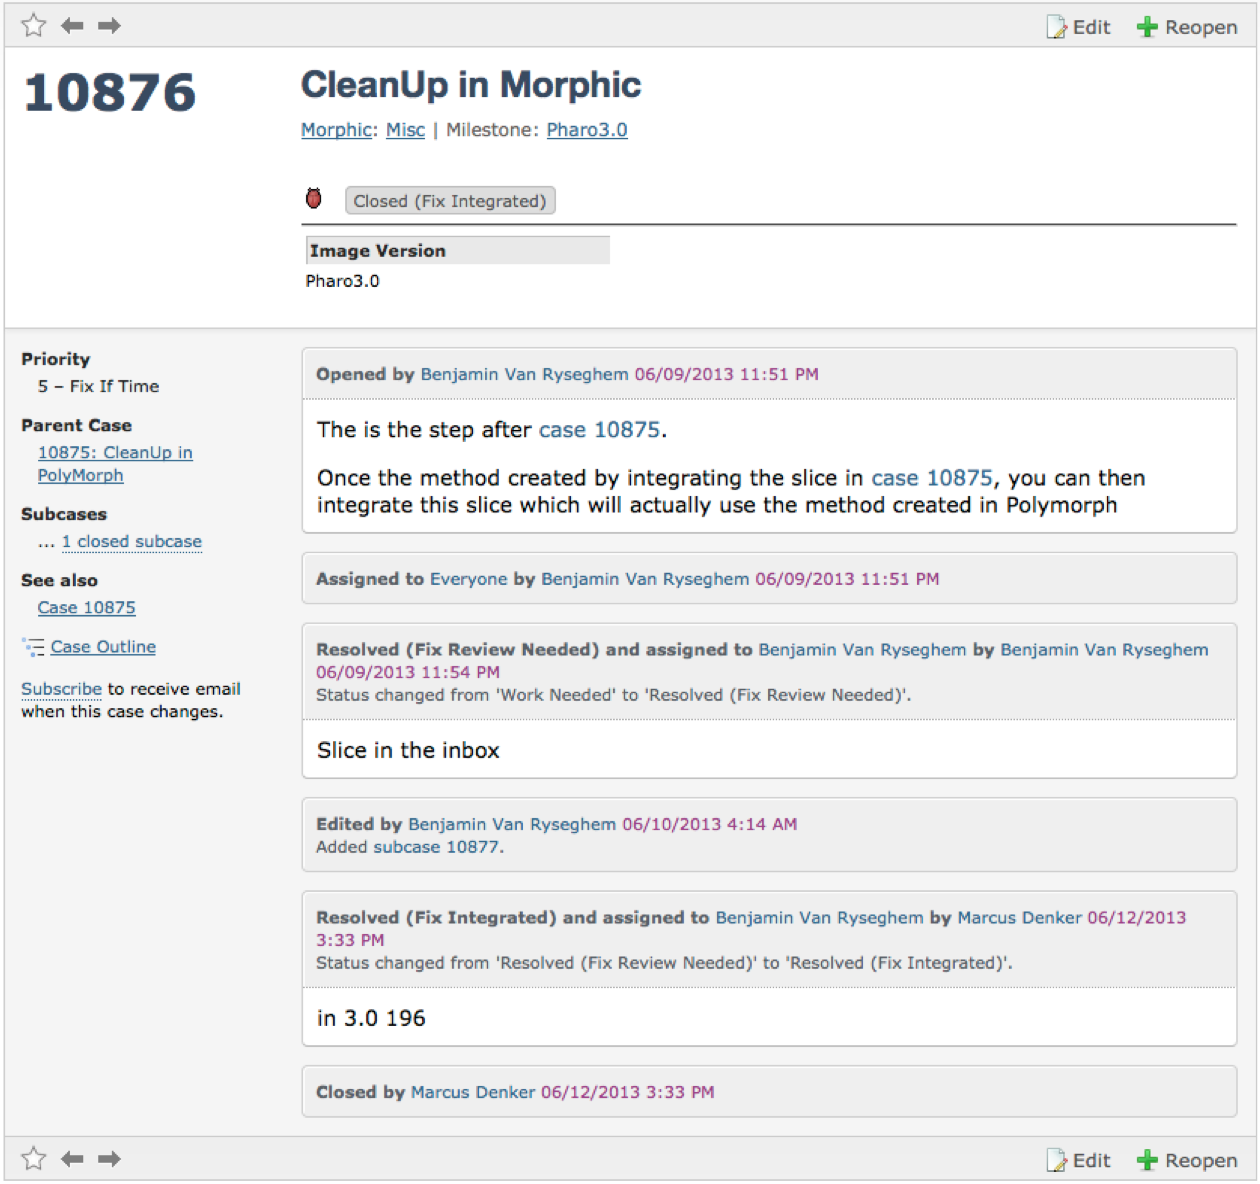
\includegraphics[width=\linewidth,trim=0 300 0 0,clip=true]{Images/fogbugz-screen.png}
\caption{Example bug report in the FogBugz bug tracking system.}
\label{fogbugz-example}
\end{figure}

Various researchers have mined and used the information stored by bug trackers to perform several types of analyses, such as identifying duplicate bug reports~\cite{Wang08a}, measuring the quality of a report~\cite{Bettenburg08}, predicting future defects~\cite{DAmb2012a}, performing traceability linking~\cite{Biss2013a}, locating features~\cite{Dit2013a}, ameliorating bug triaging decisions \cite{Anvi06a}, etc. The actual goal however is to ease the life of developers in the handling of bug reports, as part of the development process.

One problem is that bug reports are disconnected from the software system they pertain to, and it is up to the developers to restore the link between a bug report and the interested components of a system. Another problem is that bug reports, such as the one depicted in~\figref{fogbugz-example}, are displayed on individual web pages that list their properties, making them cumbersome to handle and making it also difficult to obtain a ``big picture'' of the existing open bug reports and how they overall affect the system they pertain to. Moreover, this information is stored and presented as text, which makes it hard to understand the properties of a bug report.

We present \ib, a web-based bug analytics platform, that eases the inspection, navigation, and comprehension of bug repositories, mostly by means of interactive visualizations. in*Bug provides an entry-level big picture overview to browse the content of a repository, and a detailed, complementary, interactive, and finer-grained view to understand detailed information about the bugs and the people that report them.

Other researchers have produced custom visualization of bugs, such as D'Ambros et al.~\cite{DAmb2007a,DAmb2007b} who proposed visualizations that tried to depict the complex information revolving around bugs, which are de facto independent entities when it comes to program comprehension, and not mere side effects of the evolutionary process that software systems are subjected to. While D'Ambros et al. only created standalone depictions of information taken from BugZilla, our goal with \ib is to depict live data from a bug tracker, namely FogBugz. In the near future, we plan to offer \ib as a complementary means to inspect and analyze information pertaining to bugs reported in the context of the many projects that make up the software ecosystem revolving around the Pharo\footnote{\url{http://www.pharo-project.org}} open-source community.

We present the current features of \ib, discuss its current implementation, and illustrate its usage.


\begin{figure*}[ht]
\centering
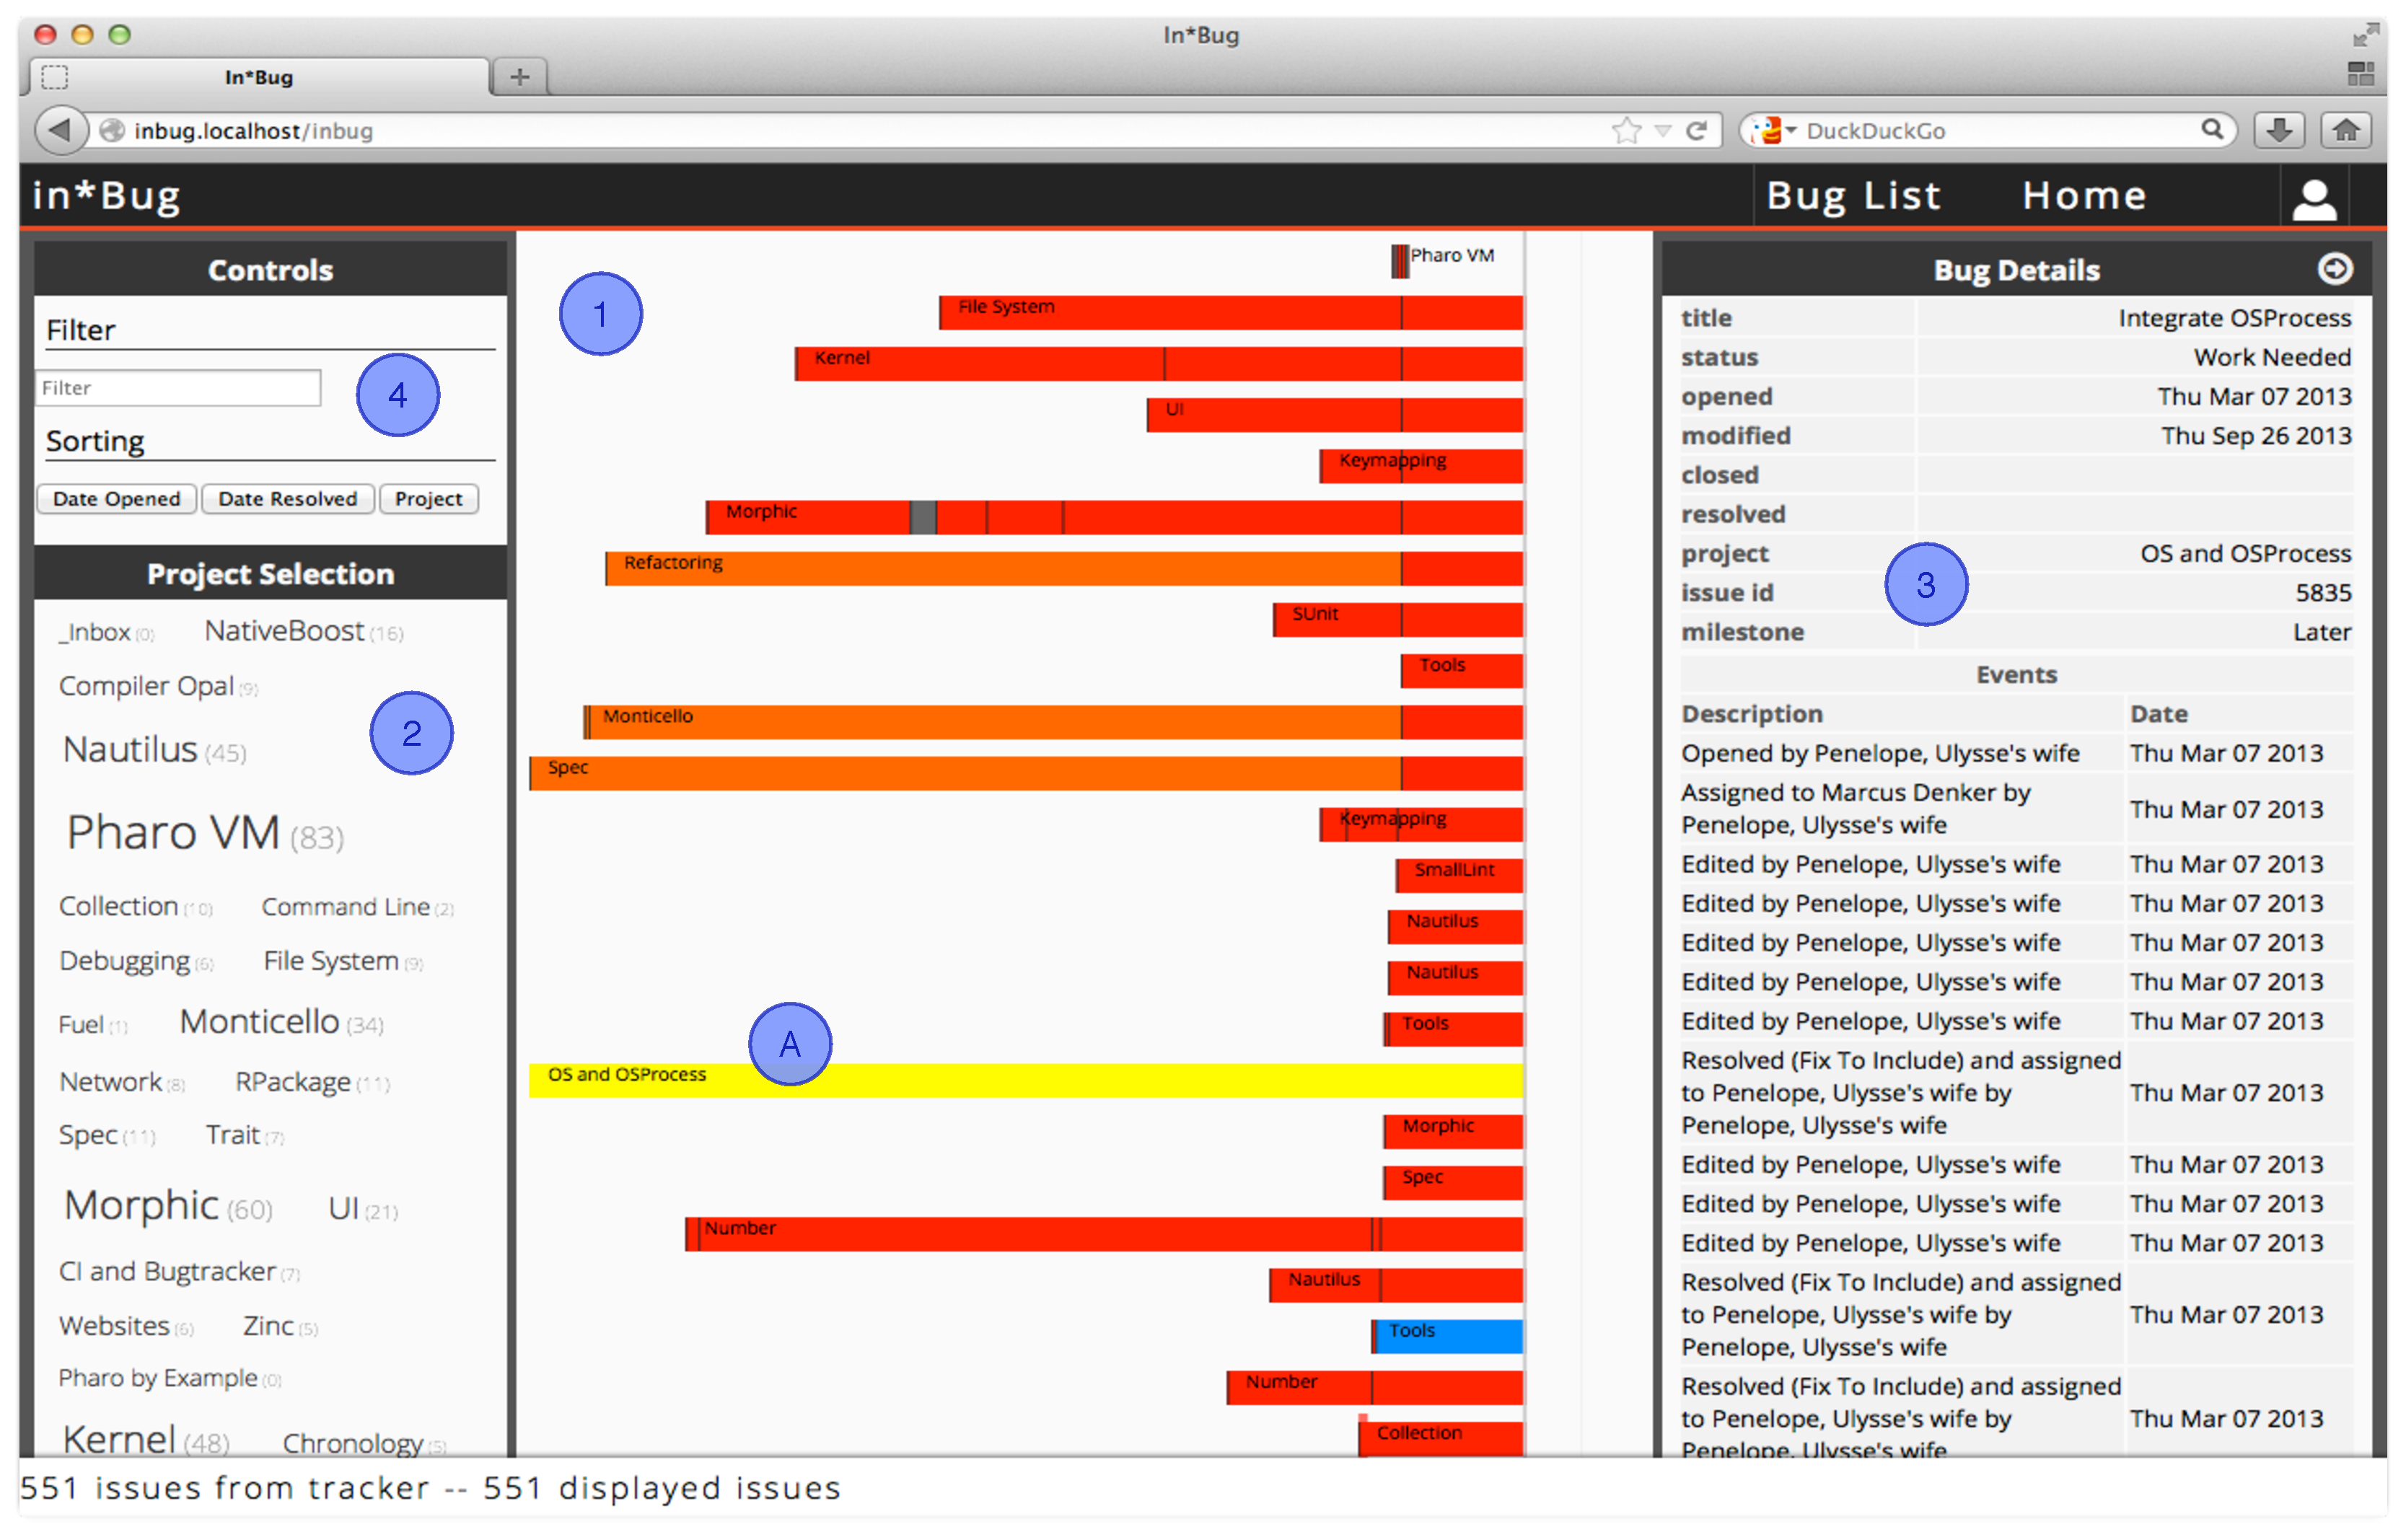
\includegraphics[width=\linewidth]{Images/inbug-list.pdf}
\caption{Main user interface of \ib}
\label{inbug}
\end{figure*}

%%%%%%%%%%%%%%%%%%%%%%%%%%
\section{in*Bug in Detail}
%%%%%%%%%%%%%%%%%%%%%%%%%%

%%%%%%%%%%%%%%%%%%%%%%
\subsection{Main view}\label{main-view}

\figref{inbug} depicts the main user interface, composed of the following panels:

{\bf Bug lifetime panel (1).} \label{bug-lifetime-panel} This view depicts the bug reports contained in the bug repository, showing their duration (as a horizontal stacked bar chart) and status (using different colors, listed in \tabref{tab-colors}).

\begin{table}[ht]
\center
\caption{Bug report event color codes}
\label{tab-colors}
\begin{tabular}{p{1.4cm} p{0.1cm} p{1.3cm} | p{1.4cm} p{0.1cm} p{1.2cm} } \hline
Active & \cellcolor{active} & orange & Work Needed & \cellcolor{work needed} & red \\
Closed & \cellcolor{closed} & gray & Resolved & \cellcolor{resolved} & dark gray \\
Working On & \cellcolor{working on} & blue & On Hold & \cellcolor{on hold} & cyan \\
Unknown & \cellcolor{unknown} & light grey & Selected & \cellcolor{yellow} & yellow \\ \hline
\end{tabular}
\end{table}

In \figref{inbug} one specific bug (marked as A) is under focus. The vertical line to the right indicates the current date, making it also clear whether a bug report is still active or not (if it is, it will touch that line). This view also helps the developer to evaluate the complexity of a bug report by summarizing the events occurred during its lifetime.

{\bf Project selection panel (2).} In this panel the user can pick the projects whose bugs she is interested in. All projects are shown as a tag cloud, where the tag size indicates the number of bugs reported for the project, also indicated with numbers between parentheses close to the name of the projects.

{\bf Details panel (3).} This panel provides all the information reported about the bug report under focus in the bug lifetime panel. This panel present both the metadata and the list of events that happened during the lifetime of a bug, including description and date of each event. The metadata is presented as extracted from the bug repository, \eg the opening date, the status, the last modification date, etc.

{\bf Filter and options panel (4).} This panel allows the user to sort and filter bugs. The three default sorting criteria order the issues by project, opening date, or date in which the bug has been resolved. The \textit{filter} field offers the possibility to enter either regular expressions or pieces of {\em Smalltalk} code as queries, allowing the users to submit custom made queries to filter bugs.

%%%%%%%%%%%%%%%%%%%%%%%%%%%%%
\subsection{Details of a bug}

\begin{figure*}[ht]
\begin{center}
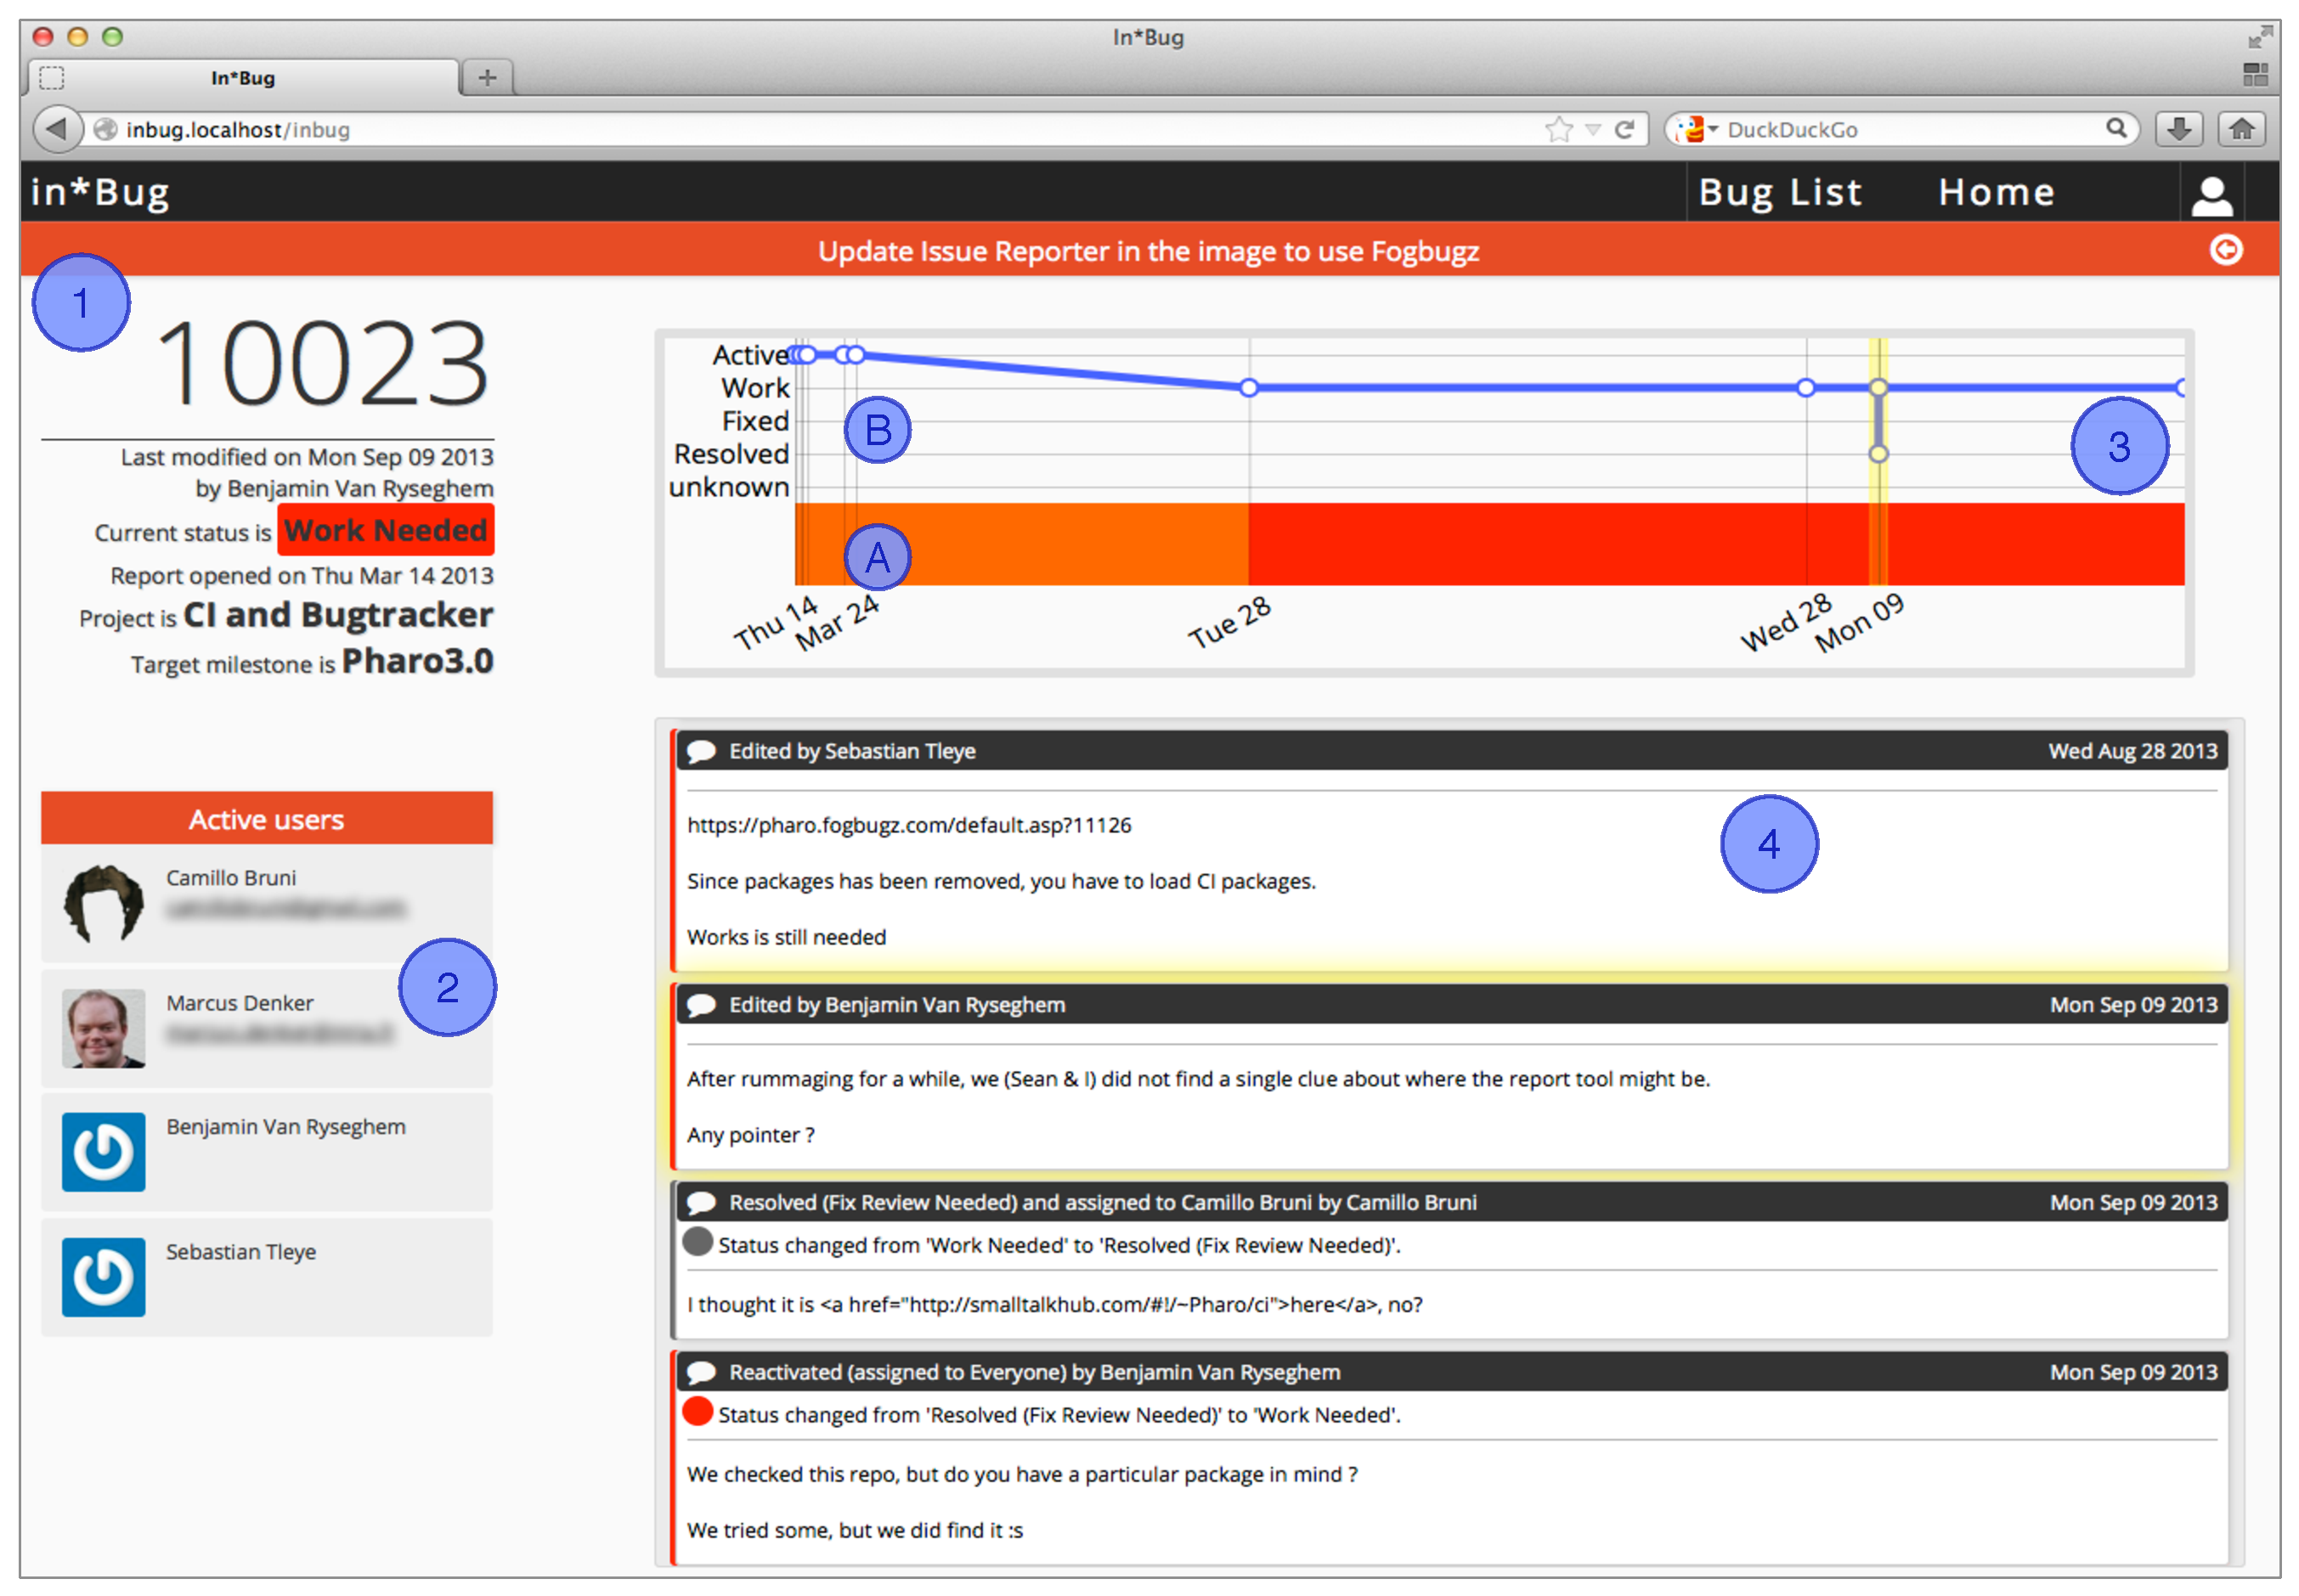
\includegraphics[width=\linewidth]{Images/details-page.pdf}
\caption{\ib details page showing the properties of a bug report}
\label{fig-inbug-home}
\end{center}
\end{figure*}

This view (see \figref{fig-inbug-home}) presents a detailed representation of a specific bug report. Each section provides a description of the element that compose the description of a defect.

\textbf{Bug Report Metadata (1).} The first panel summarizes the important metadata of the bug report: the id, the last modification, the current status, the opening date and possible closing date, the project and the target milestone for the issue resolution.

\textbf{Users List (2).} This panel gives an overview of the people involved in the evolution of the bug. In particular, the list displays the information of each user that performed an action on the issue, that was stored as an event. The details include the picture of the user, the user name and the user's email address\footnote{We obfuscated the email addresses in the figure for privacy reasons.}, to contact the people working on an issue.

\textbf{Bug Report Life Visualization (3).} This panel shows a visualization of the life of a bug report during time. The left border represents the date the issue was opened, the right border represents the moment the bug was closed, or the current date if the bug report is still active. The section (A) proposes the same visualization of the list view in the main view (\ref{main-view}), emphasising the status changes during time. The section (B) shows a line diagram where the height represents the criticality of the status (\ie fixed is the lowest and active is the hightest) and highlighting each event with a circle.

\textbf{Event Interactive View (4).} This is a list of all the events that compose a bug report. It shows the metadata of the event and whether it is an automatic event or an event generated by a user. It also detects and highlights the patches of code submitted to the tracker for the issue resolution, and provides a link to download and inspect the patch. The user can click on an event to highlight it both in the events list and in the bug report lifetime visualization. \figref{fig-event-list} shows a detail of the event list, where we can observe the three types of events: (A) shows a comment by an user; (B) shows a submitted patch. The upper left icon offers a link to the repository page of the patch; (C) indicates events automatically generated from bots in the tracker. \\
\begin{figure}[ht]
\begin{center}
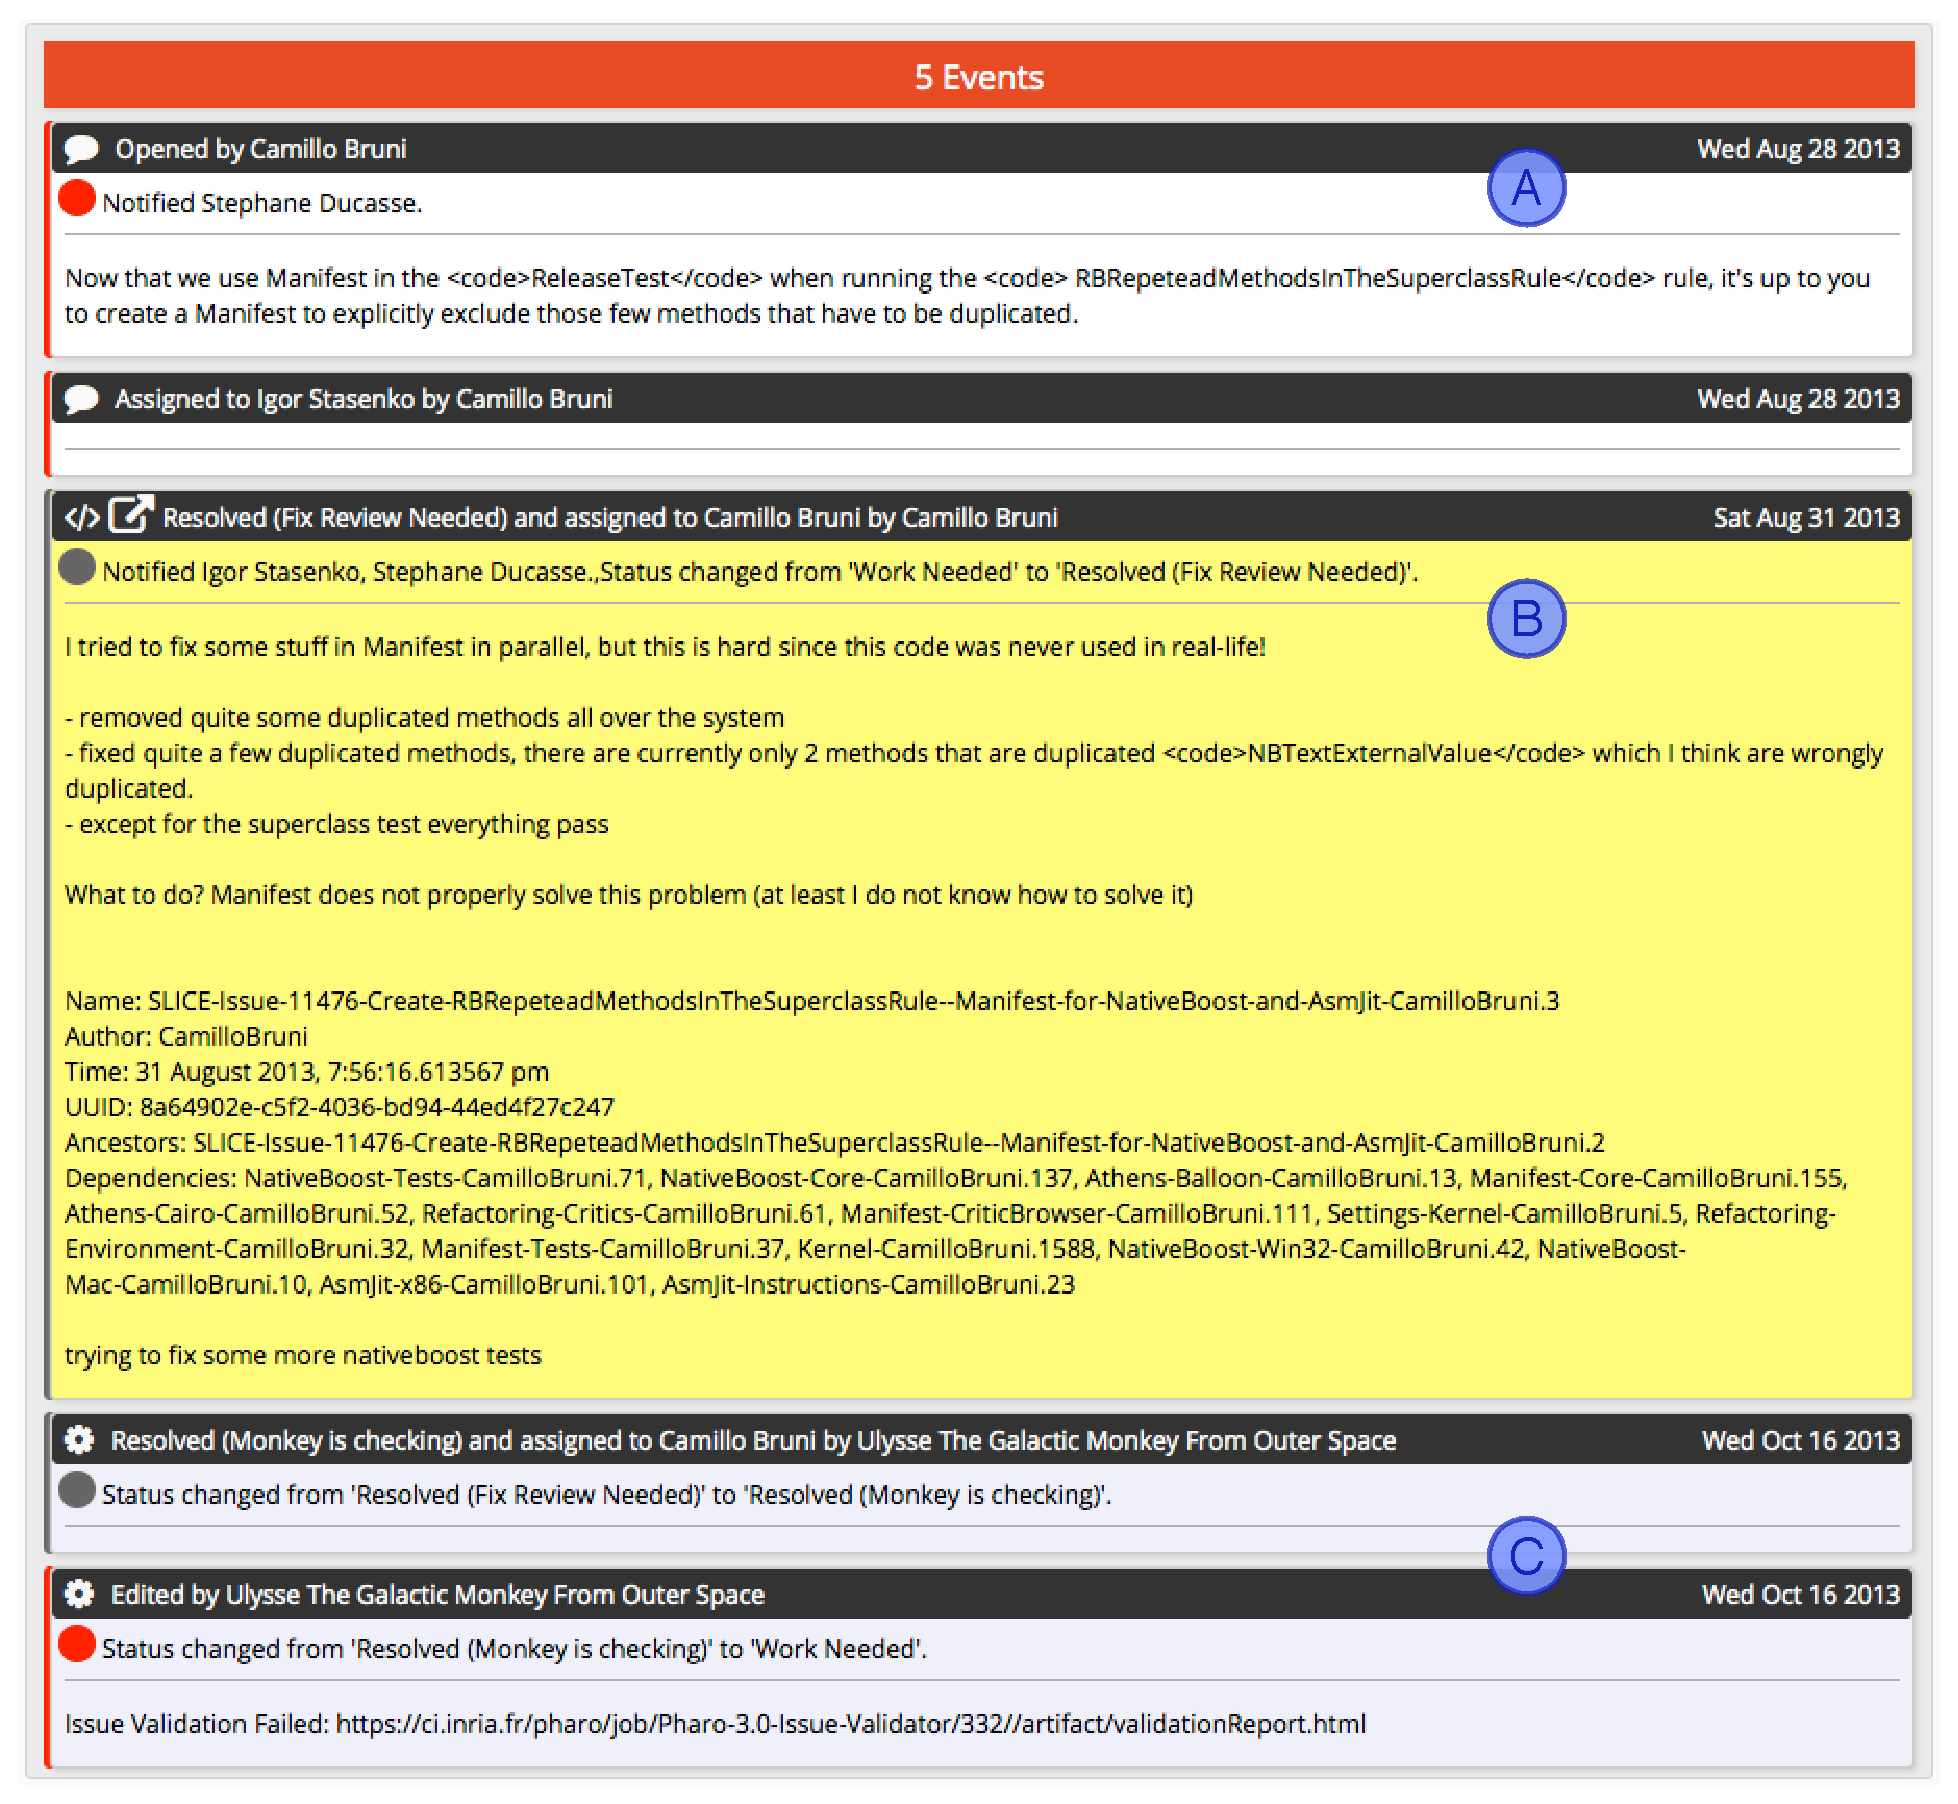
\includegraphics[width=\linewidth]{Images/event-list.pdf}
\caption{List of events in a bug report}
\label{fig-event-list}
\end{center}
\end{figure}
\indent{}Inspired by more semantically rich and elaborated views, such as Ogawa et al's storylines \cite{Ogaw2010a} or Kuhn and Stocker's storytelling timelines \cite{Kuhn2012a}, the left border of each event is colored according to the status of the event, to help the user to keep track of the evolution of the bug while inspecting the list of events.

%%%%%%%%%%%%%%%%%%%%%%%%%%%%%%%%%%%%%%%%%%%%%%
\subsection{Implementation \& Current Dataset}

\ib is a web application built on top of the \textit{Pharo Smalltalk}\footnote{\url{http://www.pharo-project.org}} environment. It uses the \textit{Seaside}\footnote{\url{http://seaside.st}} web framework to provide the data stored in a \textit{MongoDB} database and implements a \textit{RESTful API} to communicate with the client. The client interface is implemented in \textit{JavaScript} using the data manipulation and visualisation library \textit{D3.js}\footnote{\url{http://d3js.org/}}.

\ib is currently targeted at a specific FogBugz repository revolving around the Pharo ecosystem. In \tabref{tab-tracker-summary} we provide a summary of the currently available data, which has already reached considerable complexity.

\begin{table}[ht]
\center
\caption{Summary data of the \textit{Pharo} bug tracker}
\label{tab-tracker-summary}
\begin{tabular}{p{7cm} r} \hline
Number of projects & 46 \\
Number of bug reports & 8,666 \\
Number of open bug reports & 613 \\
Total number of events & 79,437 \\
Average events per issue & 9 \\ \hline
\end{tabular}
\end{table}

\ib also provides links to patches on \emph{SmalltalkHub}, a source code repository to store versioned Smalltalk code. In \figref{fig-inbug-ecosystem} we can see how these three services interact.

\begin{figure}[ht]
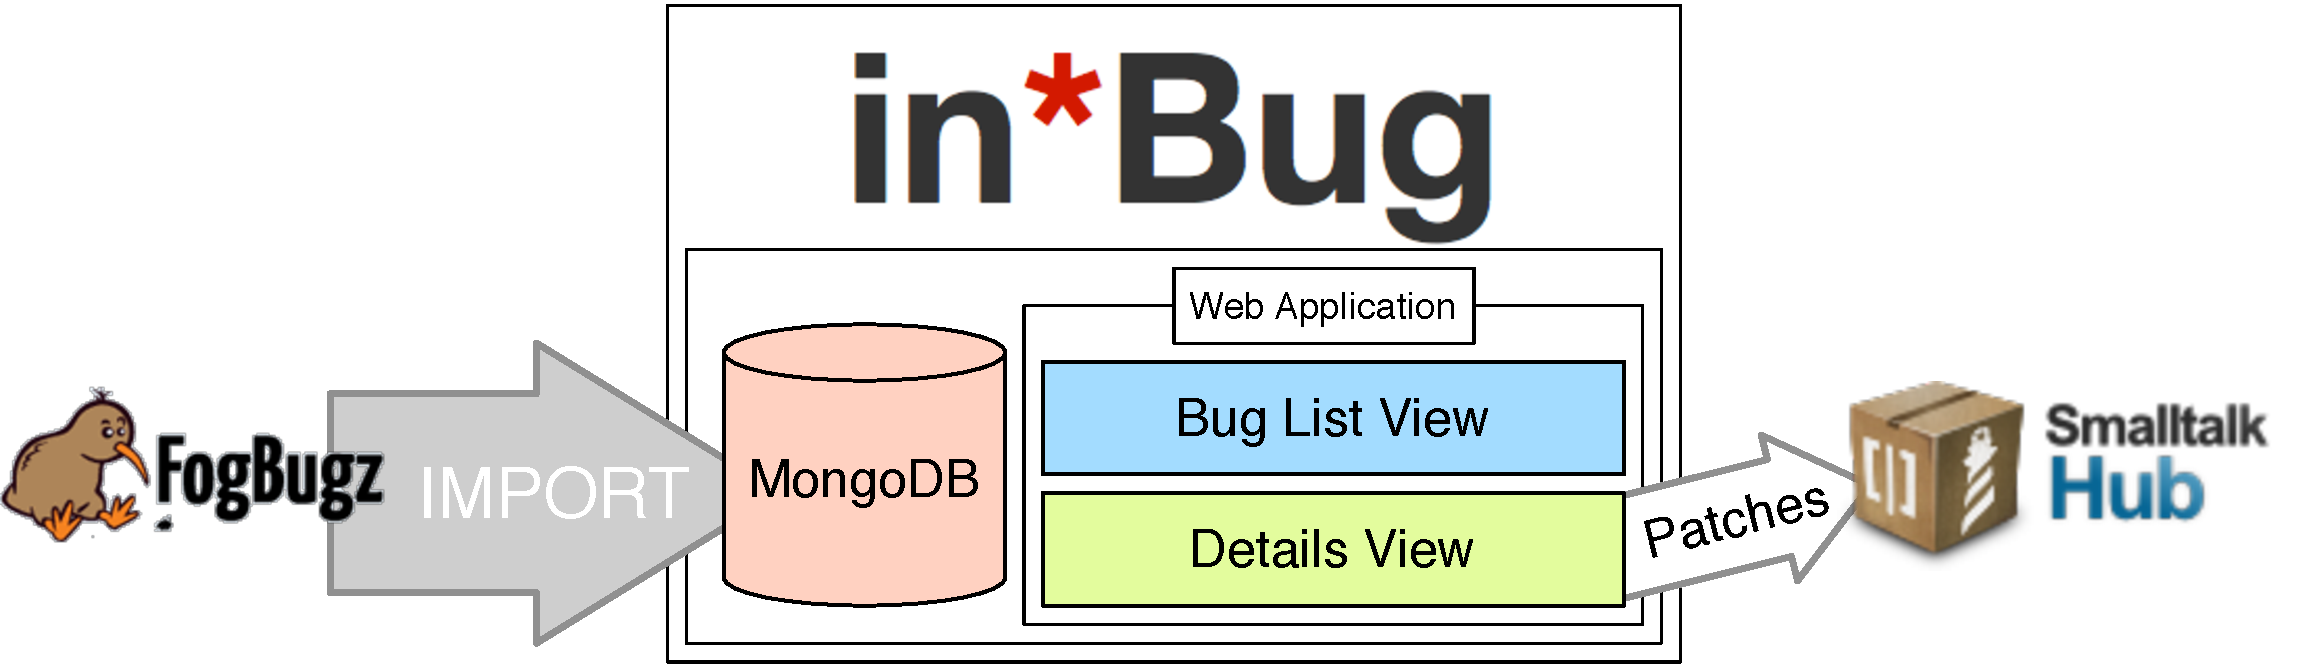
\includegraphics[width=\linewidth]{Images/inbug-ecosystem.pdf}
\caption{The interactions of \ib with the \emph{FogBugz} and \emph{SmalltalkHub} services}
\label{fig-inbug-ecosystem}
\end{figure}

%\pagebreak

The bug reports data is imported from FogBugz and stored in the MongoDB repository. The web application then loads the data and present it in the list view of the main interface. The details of a single report are presented in the details view, where the user can follow a link that leads to a patch submitted to SmalltalkHub.
%\input{application.tex}

%%%%%%%%%%%%%%%%%%%%
\section{Conclusion}
%%%%%%%%%%%%%%%%%%%%

We have presented \ib, a web-based visual analytics platform to explore the content of a bug repository. \ib allows to get a complete overview of a whole repository, as well as detailed and meaningful information on a single bug report, either through visualizations that allow to interact with the data, or with the query engine embedded in \ib that allows the user to submit queries and dialog directly with the bug reports.

We intend to provide further visualizations that describe the resume data of a single bug repository, to ease and improve the comprehension of the evolution of a software project during time.

The approach of \ib is general enough to be applied to any bug tracking system. Since we want to propose \ib as a tool for practical development, we focused on the Pharo platform and we targeted its community. We plan to improve \ib and refine the existing visualizations based on feedback obtained from Pharo users.

%Our main target is the \textit{Pharo} community, as we want to propose \ib as a tool for developing the \textit{Pharo} platform and refine the existing visualizations and improve \ib based on feedback we will get from Pharo users.

{\bf Acknowledgements.} We acknowledge the Swiss National Science foundation's support for project 146734 ``HI-SEA''.

\bibliographystyle{IEEEtran}
\bibliography{biblio}



%\begin{figure*}[ht]
%\centering
%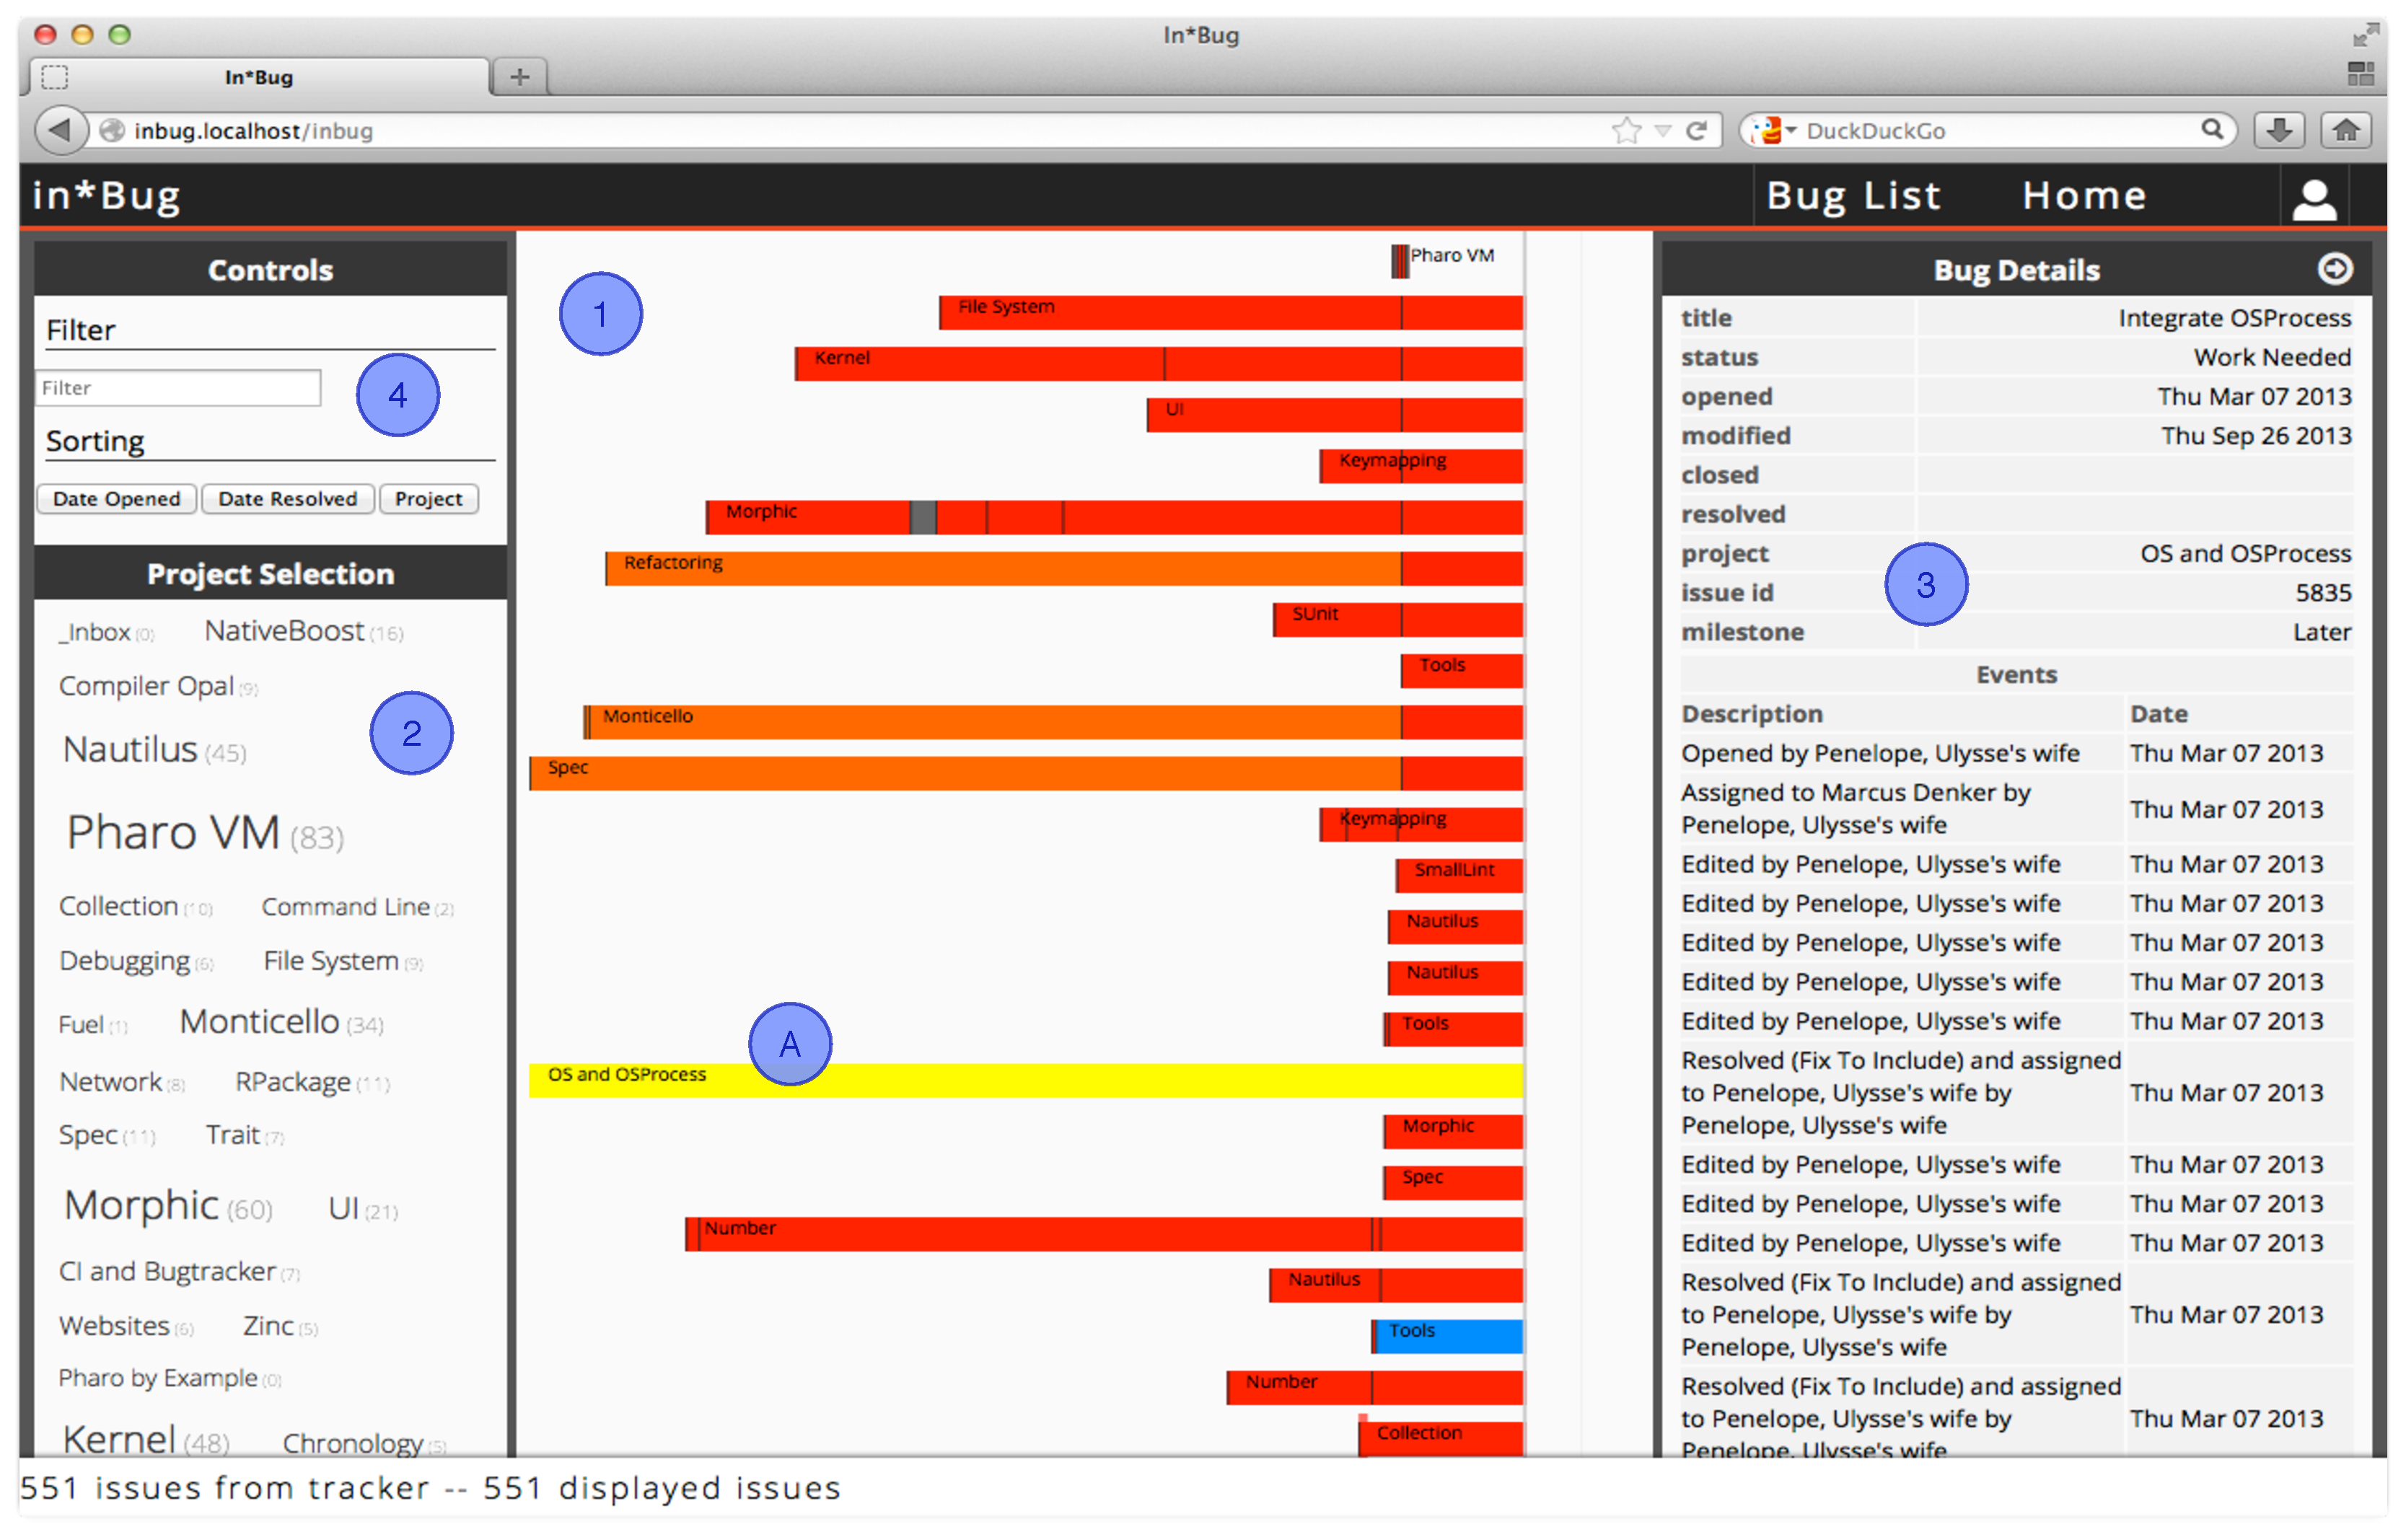
\includegraphics[width=\linewidth]{Images/inbug-list.pdf}
%\caption{Main user interface of \ib}
%\label{appendix-inbug}
%\end{figure*}

\begin{figure*}[ht]
\centering
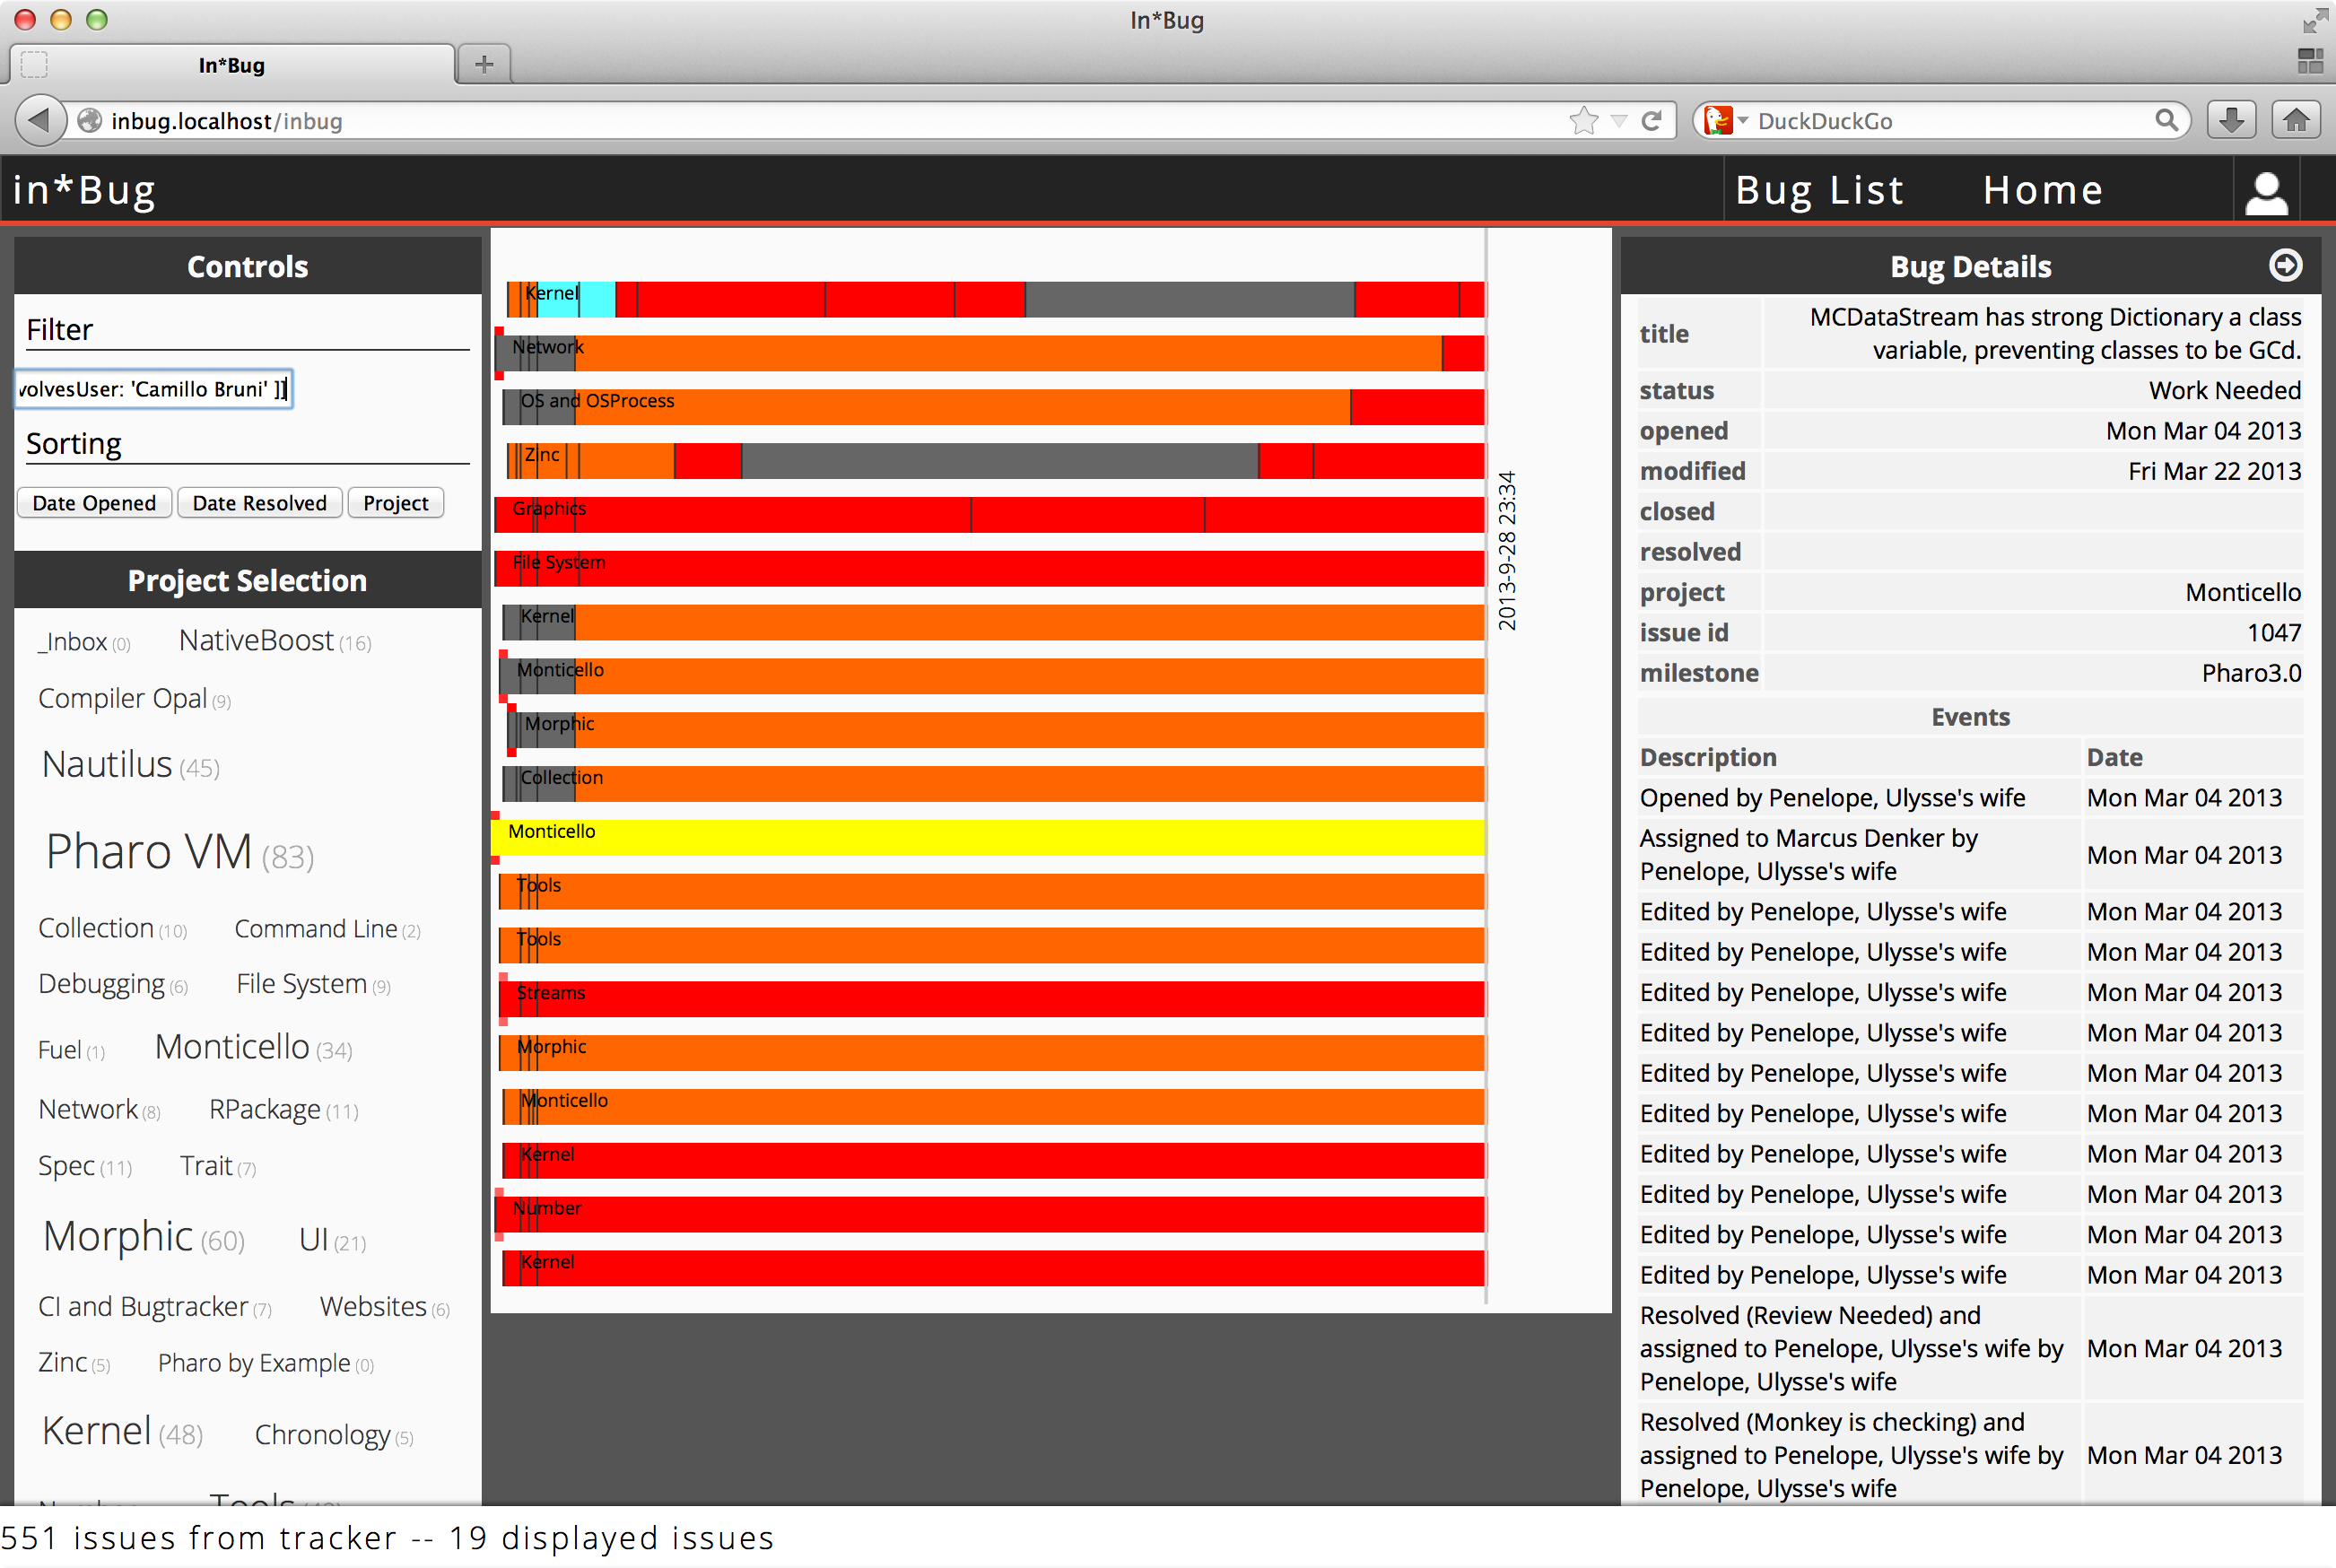
\includegraphics[width=16cm,trim=0 56 0 0,clip=true]{Images/appendix-query.png}
\caption{The result  of a Smalltalk query}
\label{appendix-query}
\end{figure*}

\newpage


\section*{Appendix - Description of the demo}

We foresee a very interactive demo, where in front of the audience we would use \ib to navigate the bug repository mentioned in \tabref{tab-tracker-summary}. In the following we do provide a plausible demo scenario, but would much rather prefer to have the audience give input on which bugs we would analyze together with them.

\begin{enumerate}

\item \textbf{Bug List View.} The beginning of the demo is to present the concepts behind the main interface of \ib. We are going to introduce the idea of a bug report as an independent entity and describe the visual representation chosen to describe a report. We then describe purpose of each panel, starting from the bug list: the possibility to examine a set of issues and their relation in terms of time collocation (see \figref{inbug}).

\item \textbf{Bug report manipulation filters.} We will show the capabilities of \ib to sort and filter the interesting reports. We will show an example of query submitted in Smalltalk, and show how we can find an interesting report with a visual inspection. \figref{appendix-query} shows the result of the query:

\begin{verbatim}
[ :each | each events size > 20 and: [
  each involvesUser: 'Camillo Bruni' ]]
\end{verbatim}

\item \textbf{Details View.} We will select a bug report to inspect and visualize its properties with the details view presented in \figref{appendix-details-view}. We will present the metadata displayed, the users involved in the report resolution, then we will see how the visualization can provide an immediate feedback on the life of a bug report, and its current status.

\begin{figure}[ht]
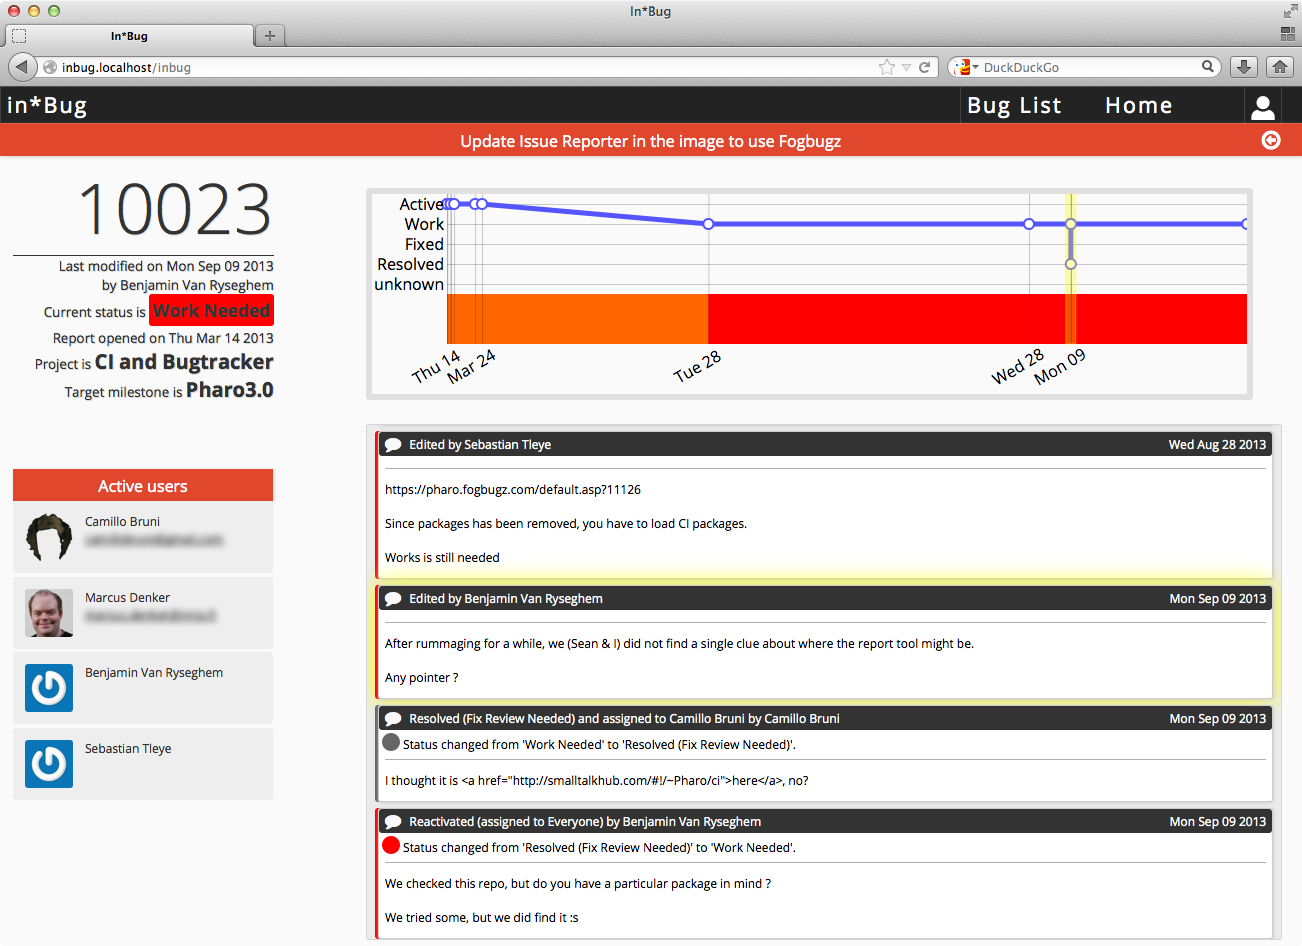
\includegraphics[width=\linewidth]{Images/details-page.png}
\caption{\ib details page showing the properties of a bug report}
\label{appendix-details-view}
\end{figure}

\item \textbf{Events and Patches.} We will examine the list of the events and the possible types of events described. We will show when \ib can detect if an event is a user comment, an automatic event or a patch submitted to fix the problem. We will show how \ib provides a link to directly retrieve the patch and examine it.

\end{enumerate}

We plan to wrap up by having a discussion about other extensions we are currently implementing, and showing off some of the directions we are currently pursuing.
